\section{Relevance feedback and query expansion}
In most collections, the same concept may be referred to using different words. This issue, known as \textit{synonymy}, has an \textbf{impact} on the \textbf{recall} of most information retrieval systems. For example, you would want a search for \textit{aircraft} to match \textit{plane} (but only for references to an airplane, not a woodworking plane), and for a search on \textit{thermodynamics} to match references to \textit{heat} in appropriate discussions. Users often attempt to address this problem themselves by manually refining a query, but in this chapter we discuss ways in which a system can help with query \textbf{refinement}, either \textbf{fully automatically} or with the \textbf{user} in the loop. 

The methods for tackling this problem split into two major classes: \textbf{global methods} and \textbf{local methods}. \textbf{Global} methods are \textbf{techniques} for \textbf{expanding} or reformulating query terms \textbf{independent} \textbf{of the query} and \textbf{results} returned from it, so that changes in the query wording will cause the new query to match other semantically similar terms. Global methods include:

\begin{itemize}
    \item Query expansion with a thesaurus or WordNet;
    \item Query expansion via automatic thesaurus generation;
    \item Techniques like spelling correction.
\end{itemize}

\textbf{Local methods} adjust a query \textbf{relative} to the \textbf{documents} that initially appear to match the query, and the basic method is \textbf{relevance feedback}.

\subsection{Relevance feedback}
The idea of \textbf{relevance feedback} (\textbf{RF}) is to \textbf{involve} the \textbf{user} in the \textbf{retrieval process} so as to improve the final result set. In particular, the user gives feedback on the relevance of documents in an initial set of results. The basic procedure is:

\begin{enumerate}
    \item The user issues a (short, simple) query;
    \item The system returns an initial set of retrieval results;
    \item The user marks some returned documents as relevant or non relevant;
    \item The system computes a better representation of the information need based on the user feedback;
    \item The system displays a revised set of retrieval results.
\end{enumerate}

The process exploits the idea that it may be difficult to formulate a good query when you don’t know the collection well, but it is easy to judge particular documents, and so it makes sense to engage in iterative query refinement of this sort. In such a scenario, relevance feedback can also be \textbf{effective} in \textbf{tracking a user’s evolving information need}: seeing some documents may lead users to refine their understanding of the information they are seeking. 

Picture \ref{relevance feedback} shows a textual IR example where the user wishes to find out about new applications of space satellites.

\begin{figure}[h!]
		\centering
		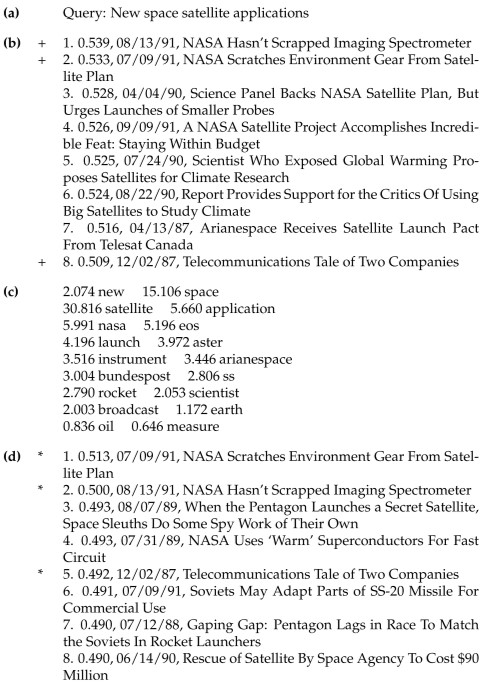
\includegraphics[scale = 2.0]{img/relevance feedback.jpg}
		\label{relevance feedback}
        \caption{Example of relevance feedback process}
\end{figure}

In the Picture:

\begin{itemize}
    \item (a) shows the initial query;
    \item (b) shows how the user marked some documents as relevant, using the +;
    \item (c) shows the terms that are used to expand the initial query, along with the weights for each term;
    \item (d) shows the revised top results. Notice that the first two documents are the same of the first top-8, while many others were not included initially.
\end{itemize}

\subsubsection{The Rocchio algorithm for relevance feedback}
The Rocchio algorithm is the classic algorithm for implementing relevance feedback in the vector space model. 

The goal of the algorithm is to find a query vector $\Vec{q}$ that maximizes the similarity with relevant documents while minimizing similarity with non-relevant documents. If $C_r$ is the set of relevant documents, and $C_{nr}$ the set of non-relevant documents, then we wish to find:

$$
\Vec{q}_{opt} = \text{arg} \max_{\Vec{q}} [\text{sim}(\Vec{q}, \mu(C_r)) - \text{sim} (\Vec{q}, \mu(C_{nr}))]
$$
, where $\mu$ is the centroid of the two sets, and it is define as $\mu(D) = \frac{1}{|D|} \sum_{d \in D} \Vec{d}$. 

Notice that if we use the cosine similarity, then the equation becomes:

$$
\Vec{q}_{opt} = \frac{1}{|C_r|} \sum_{\Vec{d}_j \in C_r} \Vec{d}_j - \frac{1}{|C_{nr}|} \sum_{\Vec{d}_j \in C_{nr}} \Vec{d}_j
$$
, i.e. the \textbf{optimal query} is the vector with \textbf{maximum difference} between the \textbf{centroids} of the relevant and non-relevant documents, as showed in Picture \ref{rocchio0}.

\begin{figure}[h!]
		\centering
		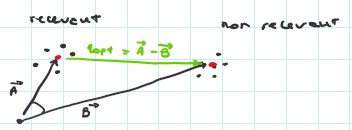
\includegraphics[scale = 2.0]{img/rocchio0.jpg}
		\label{rocchio0}
        \caption{Optimal query in Rocchio's algorithm}
\end{figure}

Notice that a strong \textbf{assumption} of this algorithm is that the full \textbf{sets of relevant and non-relevant documents are known}, which is not necessarily true in real systems. For this reason, the algorithm that was introduced and popularized in SMART system proposed to use the modified query $\Vec{q}_m$:

$$
\Vec{q}_m = \alpha \Vec{q}_0 + \beta \mu (D_r) - \gamma \mu (D_{nr})
$$
, where:

\begin{itemize}
    \item $D_r$ is the set of \textbf{known relevant document} vectors;
    \item $D_{nr}$ is the set of \textbf{known non-relevant document} vectors;
    \item $\Vec{q}_m$ is the resulting modified query vector;
    \item $\Vec{q}_0$ is the original query vector;
    \item $\alpha$, $\beta$ and $\gamma$ are weights that can be hand-chosen or set empirically;
    \item $\mu (D_r)$ and $\mu (D_{nr})$ represent, respectively, the centroid of the known relevant documents and the centroid of the known non-relevant documents.
\end{itemize}

Some notes:

\begin{itemize}
    \item Since $|D_r| << |C_r|$ and $|D_{nr}| << |C_{nr}|$, $\Vec{q}_m$ represents an \textbf{approximation} of $\Vec{q}_{opt}$;
    \item The weights control the balance between trusting the judged document set versus the query: if we have a lot of judged documents, we would like a higher $\beta$ and $\gamma$;
    \item Starting from $q_0$, the \textbf{new query moves} you some distance \textbf{toward} the \textbf{centroid} of the \textbf{relevant documents} and some distance \textbf{away} from the \textbf{centroid} of the \textbf{non-relevant documents};
    \item Negative term weights are ignored, i.e. they are set to 0.
\end{itemize}

Picture \ref{rocchio2} shows an application of Rocchio's algorithm: after some documents are labeled as relevant and non-relevant, the initial query vector is moved in response to this feedback

\begin{figure}[h!]
		\centering
		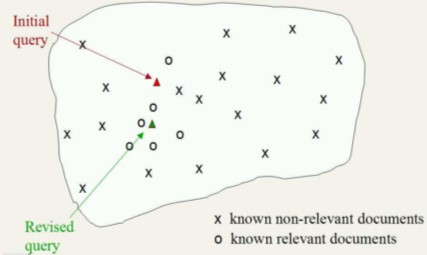
\includegraphics[scale = 2.0]{img/rocchio2.jpg}
		\label{rocchio2}
        \caption{Example of Rocchio's algorithm}
\end{figure}

\textbf{Relevance feedback} can \textbf{improve} both \textbf{recall} and \textbf{precision}. But, in practice, it has been shown to be most useful for increasing recall in situations where recall is important. This is partly because the technique expands the query, but it is also partly an effect of the use case: when they want high recall, users can be expected to take time to review results and to iterate on the search. 

\textbf{Positive feedback} also turns out to be \textbf{much more valuable} than \textbf{negative feedback}, and so most IR systems set $\gamma < \beta$. Reasonable values might be $\alpha = 1$, $\beta = 0.75$, and $\gamma = 0.15$. In fact, many systems allow only positive feedback, which is equivalent to setting $\gamma = 0$. 

In general, the \textbf{disadvantages} of relevance feedback are the following:

\begin{itemize}
    \item It is \textbf{expensive}: it creates long modified queries,as the resulting vectors are less sparse, which are expensive to process;
    \item Users are reluctant to provide explicit feedback;
    \item It's often hard to understand why a particular document was retrieved after applying relevance feedback.
\end{itemize}

\subsubsection{Pseudo-relevance feedback}
\textbf{Pseudo relevance feedback} provides a \textbf{method} for \textbf{automatic local analysis}. It \textbf{automates} the \textbf{manual part of relevance feedback}, so that the user gets improved retrieval performance without an extended interaction. 

The method is to do normal retrieval to find an \textbf{initial set of most relevant documents}, to then \textbf{assume} that the \textbf{top-$k$} ranked documents are \textbf{relevant}, and finally to do relevance feedback as before under this assumption. This automatic \textbf{technique} mostly \textbf{works}, but can go horribly wrong for some queries, due to the \textit{query drift} problem.

\subsection{Query expansion}
In relevance feedback, users give additional input on documents (by marking documents in the results set as relevant or not), and this input is used to re-weight the terms in the query for documents. In \textbf{query expansion} on the other hand, users give additional input on query words or phrases, possibly \textbf{suggesting additional query terms}. Some search engines (especially on the web) suggest related queries in response to a query (\textit{Also try..}); the users then opt to use one of these alternative query suggestions.

The central question in this form of query expansion is \textbf{how to generate alternative or expanded queries for the user}. The most common form of query expansion is \textbf{global analysis} (i.e. \textbf{not query dependent}), using some form of \textbf{thesaurus}. For each term $t$ in a query, the \textbf{query} can be automatically \textbf{expanded} with \textbf{synonyms} and \textbf{related words} of $t$ from the thesaurus. Use of a thesaurus can be combined with ideas of \textbf{term weighting}: for instance, one might weight added terms less than original query terms.

Methods for building a thesaurus for query expansion include:

\begin{itemize}
    \item Use of a controlled \textbf{vocabulary} maintained by human editors;
    \item A \textbf{manual thesaurus}, i.e. a set of synonyms;
    \item An \textbf{automatically derived thesaurus}, formed by exploiting co-occurrence statistics over collections of documents and word embeddings;
    \item Using \textbf{query log mining}, i.e. exploiting the manual query reformulations, the session analysis and the co-clicks of other users to make suggestions to a new user. This requires a huge query volume, and is thus particularly appropriate to web search.
\end{itemize}

Thesaurus-based query expansion has the \textbf{advantage} of \textbf{not requiring any user input}. Use of query expansion generally \textbf{increases} \textbf{recall}, but it may significantly \textbf{reduce} the \textbf{precision}, particularly when the query contains ambiguous term. In this sense, a domain specific thesaurus is required: general thesauri and dictionaries give far too little coverage of the rich domain-particular vocabularies of most scientific fields. It is widely used in many science and engineering fields. Moreover, it is very expensive to create a manual thesaurus and to maintain it over time.

\subsubsection{Automatic thesaurus generation}
As we introduced before, an automatic thesaurus can be exploited for query expansion. 

Before analyzing how an automatic thesaurus can be generated, we now focus on how we can represent the \textbf{words} as \textbf{vectors}. Notice that this task is particularly useful, since we can exploit the vector representations in order to compute similarity between words. One possibility is to consider a \textbf{one-hot representation} of terms, i.e. each term is represented by an extremely sparse vector $v \in \mathbb{R}^N$, where $N$ is the lexicon size, and $v[i] = 1$ if the term is equal to the one in the lexicon, 0 otherwise. Clearly, this representation is not very suitable, since:

\begin{itemize}
    \item It results in very high dimensional vectors;
    \item It does not provide a notion of similarity between vectors: e.g. \textit{car} and \textit{automobile}, despite being two similar words, are orthogonal vectors.
\end{itemize}

A possible solution is to \textbf{learn to encode similarity in the vectors} themselves, and in particular by representing \textbf{words} by their \textbf{context}. In this case, a word's meaning is given by the words that frequently appear close-by, and in order to represent a word, we use many contexts of it.

This notion is particularly useful for \textbf{automatic thesaurus generation}, whose attempt is to generate a thesaurus by analyzing a collection of documents. There are two main approaches:

\begin{enumerate}
    \item Exploit \textbf{word co-occurrence}. We say that words co-occurring in a document or paragraph are likely to be in some sense similar or related in meaning, and simply count text statistics to find the most similar words;
    \item Use a shallow \textbf{grammatical analysis} of the text and to exploit grammatical relations or grammatical dependencies. For example, we say that entities that are grown, cooked, eaten, and digested, are more likely to be food items.
\end{enumerate}

\begin{figure}[h!]
		\centering
		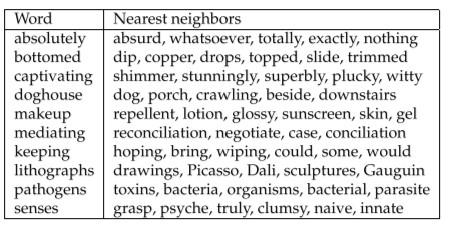
\includegraphics[scale = 2.0]{img/automatic thesaurus.jpg}
		\label{automatic thesaurus}
        \caption{Example of an automatically generated thesaurus}
\end{figure}

\textbf{Simply} using\textbf{ word co-occurrence} is \textbf{more robust} (it cannot be misled by parser errors), but using \textbf{grammatical relations is more accurate}. 

The simplest way to compute a co-occurrence thesaurus is based on \textbf{term-term similarities}. We begin with a \textbf{term-document matrix} $A$, where each cell $A_{t,d}$ is a weighted count $w_{t,d}$ for term $t$ and document $d$, with weighting so $A$ has length-normalized rows. Notice that the dimensionality of $A$ is $M \times N$, where $M$ is the size of the lexicon, and $N$ is the size of the collection, i.e. the number of documents. If we then calculate $C = AA^T$, then $C_{u,v}$ is a \textbf{similarity score} between terms $u$ and $v$, with a \textbf{larger} number being \textbf{better}. 

While some of the thesaurus terms are good or at least suggestive, others are marginal or bad. Term ambiguity easily introduces irrelevant statistically correlated terms. For example, a query for \textit{Apple computer} may expand to \textit{Apple red fruit computer}. In general these thesauri suffer from both \textbf{false positives} and \textbf{false negatives}. Moreover, since the terms in the automatic thesaurus are highly correlated in documents anyway (and often the collection used to derive the thesaurus is the same as the one being indexed), this form of \textbf{query expansion} \textbf{may not retrieve many additional documents}. 

Another very important way to compute a co-occurrence thesaurus is to use \textbf{word embeddings}: we build a \textbf{dense vector for each word}, with the property that it is similar to vectors of words that appear in similar context. In particular, we can measure \textbf{similarity} between documents by using the \textbf{dot product}. A famous framework that is used for learning word vectors is \textbf{Word2vec}, which works as follows:

\begin{itemize}
    \item A large corpus of text is provided as input to the model;
    \item Each word is the represented by a vector;
    \item The model goes through each position $t$ in the text, which has a center word $c$ and a list of context words $o$ (usually not so large): the similarity between the vectors $c$ and each context word $o$ is used to calculate the probability of $o$ given $c$ (or vice-versa), as showed in Picture \ref{word2vec}. 

    \begin{figure}[h!]
		\centering
		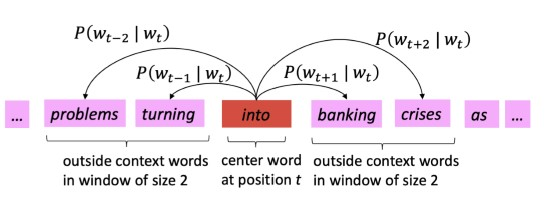
\includegraphics[scale = 2.0]{img/word2vec.jpg}
		\label{word2vec}
        \caption{Example of windows and process for computing the probabilities}
    \end{figure}
    
    Then, the model keeps adjusting the word vectors to maximize this probability.
\end{itemize}

In other words, the goal of Word2vec is to train a \textbf{Neural Network} on a large corpus of pairs $(c,o)$, i.e. center and context terms pairs. An example of training samples is provided in Picture \ref{word2vec2}, while Picture \ref{word2vec3} shows the Neural Network that is used for implementing Word2vec.

\begin{figure}[h!]
		\centering
		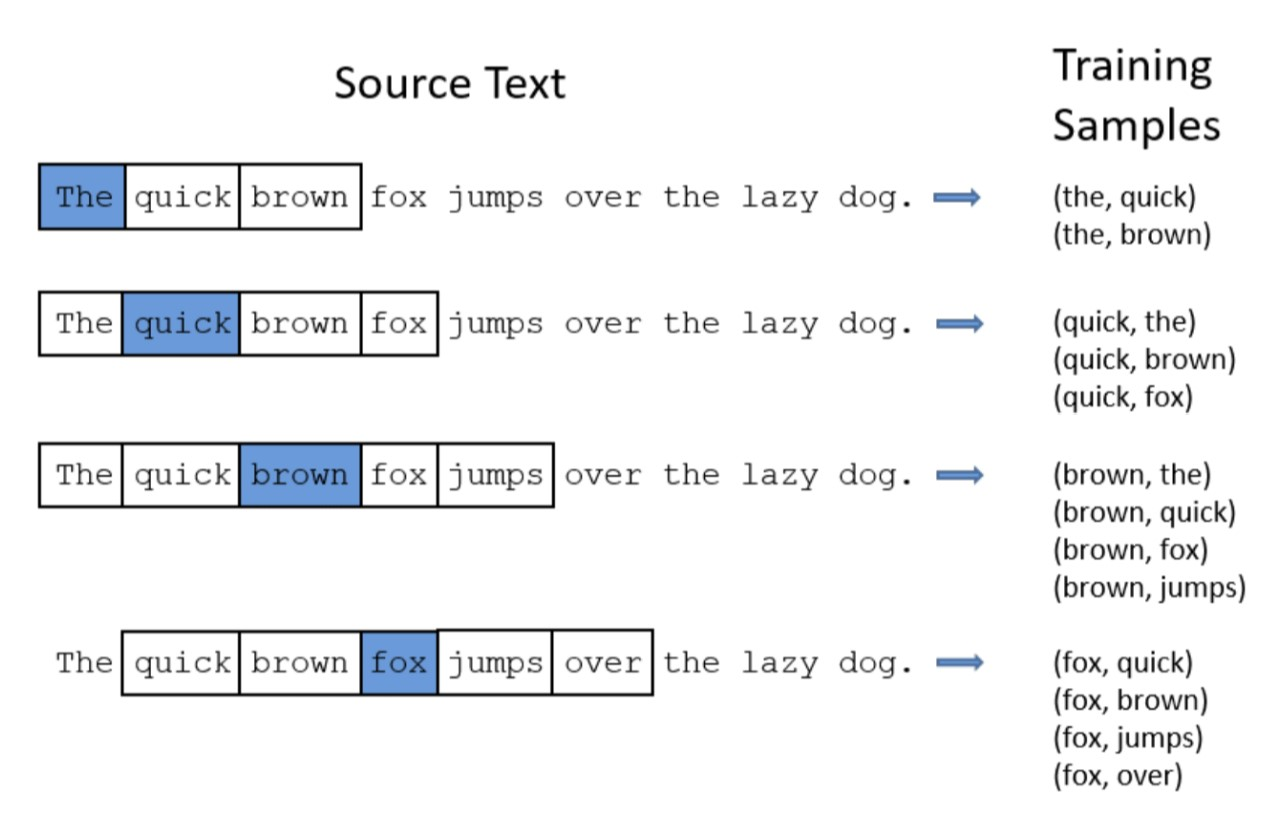
\includegraphics[scale = 0.6]{img/word2vec2.jpg}
		\label{word2vec2}
        \caption{Example of training samples}
\end{figure}

\begin{figure}[h!]
		\centering
		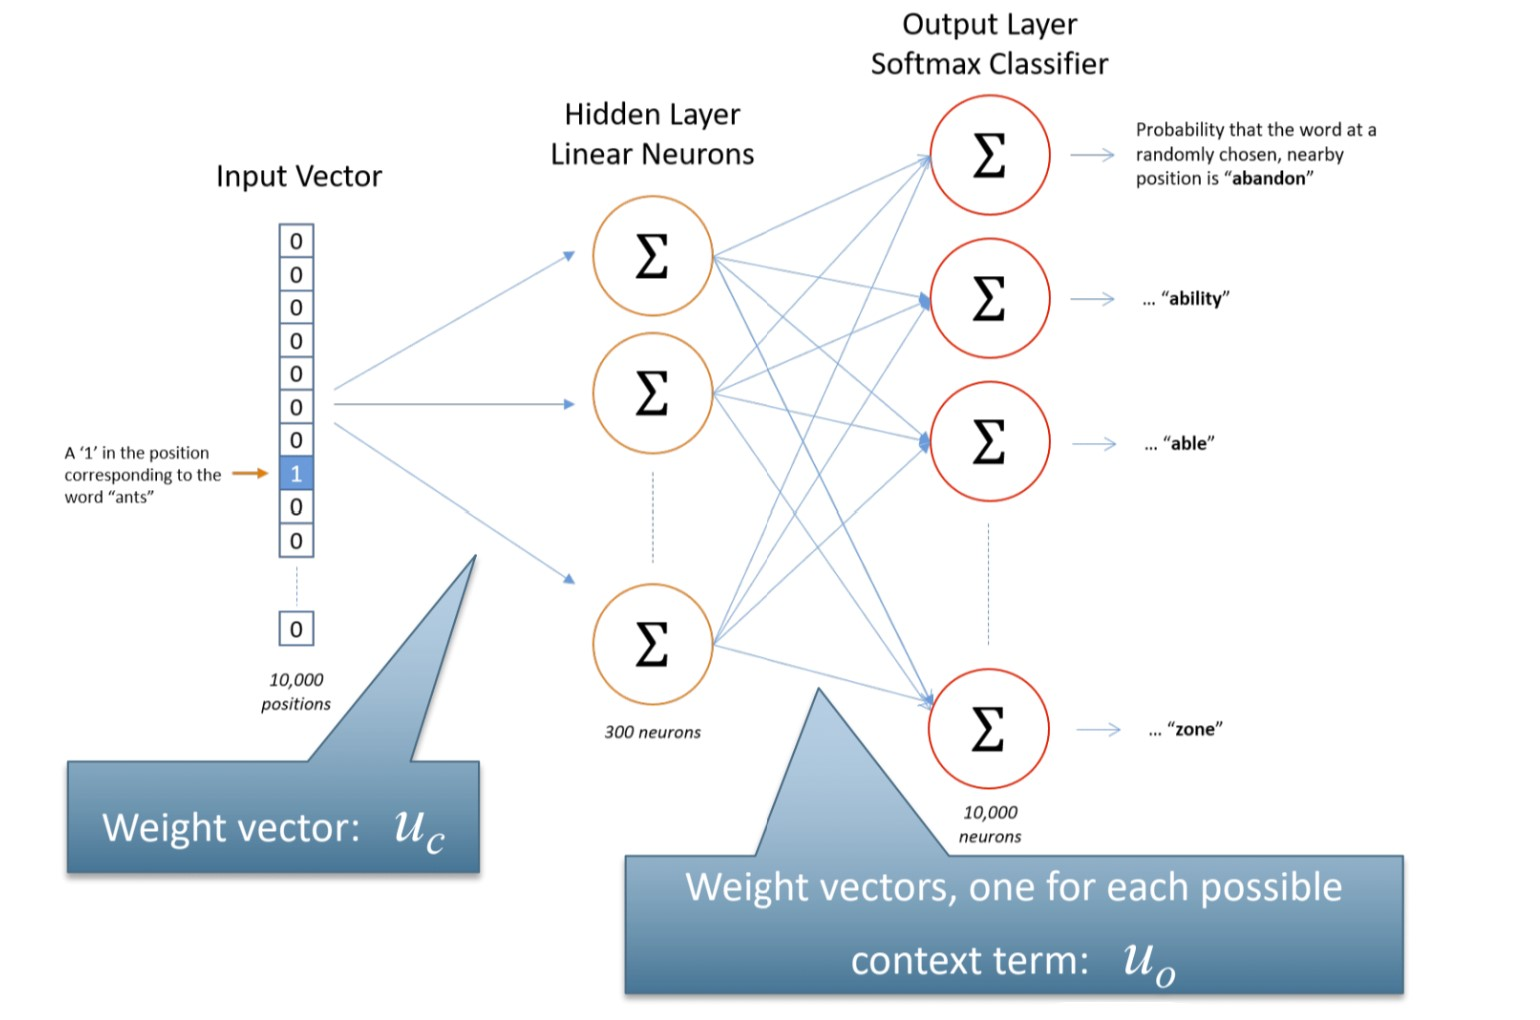
\includegraphics[scale = 1.0]{img/word2vec3.jpg}
		\label{word2vec3}
        \caption{Neural Network of Word2vec}
\end{figure}

As we can see, the Network receives in input a vector in which there's a 1 in the position corresponding to the center word $c$, and for each term in the lexicon, it produces a probability that the word at a randomly chosen, nearby position is the term itself. Notice that the output layer is represented by a \textbf{Softmax classifier}, whose goal is to map a real number (in this case the similarity between vectors) to a probability distribution. In particular, for each word $w$, we use two different vectors:

\begin{itemize}
    \item $v_w$ when $w$ is a center word;
    \item $u_w$ when $w$ is a context word.
\end{itemize}

Then, for a center word $c$ and a context word $o$, we compute:

$$
P(o | c) = \frac{\exp{u_o^T v_c}}{\sum_{w \in V} \exp{u_w^T v_c}}
$$

Then, network minimizes the \textbf{cross-entropy} using Stochastic Gradient Descent. 

In the case of query expansion, Word2vec can be used by expanding a query retrieving the k-nearest neighbors w.r.t. the term-vector similarity. The method works as follows:

\begin{itemize}
    \item Each query is represented by a set of terms: $q = \{ t_1, t_2, .., t_m \}$;
    \item We build a set of $m \times k$ candidate terms: $C = \bigcup_{t \in q} \text{k-NN} (t)$;
    \item Terms in $C$ are sorted on the basis of the following score: $\text{AvgSim}(t,q) = \frac{1}{|q|} \sum_{t_i \in q} \text{cosine}(t, t_i)$, and the top-$k$ candidates are finally selected as expansion terms.
\end{itemize}

